\chapter{Tool}
\label{Chapt:Tool}

%===============================================================================
% VERBOSE MODE
%===============================================================================

\section{Verbose mode}
\label{Sec:Verbose}

This module shows verbose information about the progress of the
JIT compiler. It prints one line for each generated trace. This module
is useful to see which code has been compiled or where the compiler
stops and falls back to the interpreter.

Example usage:

\begin{lstlisting}
  mad -jv -e "for i=1,1000 do for j=1,1000 do end end"
  mad -jv=myapp.out myapp.mad
\end{lstlisting}
To redirect the output to a file, pass a
filename as an argument (use '-' for stdout) or set the environment
variable LUAJIT\_VERBOSEFILE. The file is overwritten every time the
module is started.

The output from the second example could look like this:

\begin{center}
[TRACE   1 myapp.mad:1 loop]

[TRACE   2 (1/3) myapp.mad:1 $->$ 1]
\end{center}

The first number in each line is the internal trace number. Next is
the file name ('myapp.mad') and the line number (':1') where the
trace has started. Side traces also show the parent trace number and
the exit number where they are attached to in parentheses ('(1/3)').
An arrow at the end shows where the trace links to ('$->$ 1'), unless
it loops to itself.

In this case the inner loop gets hot and is traced first, generating
a root trace. Then the last exit from the 1st trace gets hot too
and triggers the generation of the 2nd trace. The side trace follows the
path along the outer loop and \textit{around} the inner loop, back to its
start, and then links to the 1st trace.

Aborted traces are shown like this:
\begin{center}
[TRACE --- foo.mad:44 -- leaving loop in root trace at foo:mad:50]
\end{center}

Trace aborts are quite common, even in programs which
can be fully compiled. The compiler may retry several times until it
finds a suitable trace. This doesn't work with features that are
not-yet-implemented (NYI error messages). LuaJIT simply falls back to the
interpreter. This may not matter at all if the particular trace is not very high
up in the CPU usage profile, plus the interpreter is quite fast, too.

%===============================================================================
% PROFILER
%===============================================================================

\section{Profiler}
\label{Sec:Profiler}

This module is a simple command line interface to the built-in
low-overhead profiler of LuaJIT. The lower-level API of the profiler
is accessible via the "jit.profile" module or the LuaJIT\_profile\_* C API.

Example usage:
\begin{lstlisting}
  mad -jp myapp.mad
  mad -jp=s myapp.mad
  mad -jp=-s myapp.mad
  mad -jp=vl myapp.mad
  mad -jp=G,profile.txt myapp.mad
\end{lstlisting}
The following dump features are available:
 \begin{itemize}%[label={--}]
  \item \textbf{f} - Shows function name (Default mode).
  \item \textbf{F} - Shows function name with module prepend.
  \item \textbf{l} - Shows line granularity ('module':'line').
  \item \textbf{\textless number\textgreater} - Stack dump depth (callee\textless caller - Default: 1)
  \item \textbf{-\textless number\textgreater} - Inverse stack dump depth (caller\textgreater callee).
  \item \textbf{s} - Split stack dump after first stack level. Implies $\mid depth\mid$
  \textgreater= 2.
  \item \textbf{p} - Show full path for module names.
  \item \textbf{v} - Show VM states (See bellow).
  \item \textbf{z} - Show zones (See bellow).
  \item \textbf{r} - Show raw sample counts (Default: percentages).
  \item \textbf{a} - Annotate excerpts from source code files.
  \item \textbf{A} - Annotate complete source code files.
  \item \textbf{G} - Produce raw output suitable for graphical tools (See bellow).
  \item \textbf{m\textless number\textgreater} - Minimum sample percentage to be shown (Default: 3).
  \item \textbf{i\textless number\textgreater} - Sampling interval in milliseconds (Default: 10).
 \end{itemize}

 Many of those options can be activated at ones.\\

We can also use this module programmatically like in the example below. The
\emph{start} function can take 2 arguments, the list of options (describe above)
and the output file.
\begin{lstlisting}[style=LuaStyle]
local prof = require"jit.p"
prof.start("vf", "file.txt")
  -- Code to analyze here
prof.stop()
\end{lstlisting}

\subsubsection{VM states:}
This option allows to shows the time spent in which state of the VM.
States can be of the following types :

\{Compiled - Interpreted - C code - Garbage Collector - JIT Compiler\} \\

\subsubsection{Zone:}
Statistics can be grouped in user defined zone. Below is an example a such a
definition.
\begin{lstlisting}
    local zone = require("jit.zone")
    zone("MyZone")
      -- Lua code here
    zone()
\end{lstlisting}

\subsubsection{Graphical tools:}
This option can be used to graphically show the dump in a nice image format
(see Appendix \ref{Apendix:fl})

Figure \ref{fig:profiler} shows two different outputs of the run of the
\emph{Sequence} tests presented in Part \ref{Part:mad}. On the left we can see
the default mode of the profiler with the percentage of time spent per function.
On the right we see the percentage of time spent per VM states (the \emph{v} mode).

\begin{figure}[H]
    \centering
    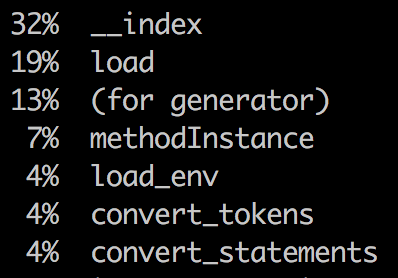
\includegraphics[height=3.5cm]{luajit/images/chapter4/profiler-1.png}
    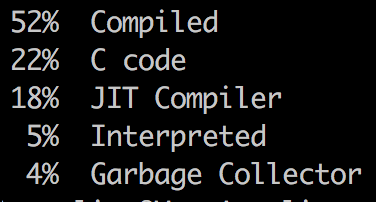
\includegraphics[height=3.5cm]{luajit/images/chapter4/profiler-2.png}
    \caption{Screenshots of the profiler outputs}
    \label{fig:profiler}
\end{figure}

%===============================================================================
% DUMP MODE
%===============================================================================

\section{Dump mode}
\label{Sec:Dump-mode}


%===============================================================================
% How to use it
%===============================================================================


\subsection{How to use it}
\label{Subsec:dump-usage}

This module can be used to debug the JIT compiler itself or to analyze its
behavior when running a particular code. It dumps the
code representations and structures used in various compiler stages. Some
concrete examples of its usage can be found in Chapter \ref{Chapt:MO}.

Example usage:
\begin{lstlisting}
  mad -jdump -e "
    local x=0
    for i=1,1e6 do x=x+i end
    print(x)
  "
  mad -jdump=im -e "
    for i=1,1000 do
      for j=1,1000 do end
    end
  " | less -R
  mad -jdump=is myapp.mad | less -R
  mad -jdump=-b myapp.mad
  mad -jdump=+aH,myapp.html myapp.mad
  mad -jdump=ixT,myapp.dump myapp.mad
\end{lstlisting}
The first argument specifies the dump mode. The second argument gives
the output file name. Default output is to stdout, unless the environment
variable LUAJIT\_DUMPFILE is set. The file is overwritten every time the
module is started. Different features can be turned on or off with the dump mode.
If the mode starts with a '+', the following features are added to the default
set of features; a '-' removes them. Otherwise the features are replaced.\\
The following dump features are available (* marks the default):

\begin{itemize}
  \item \textbf{t *} - Print a line for each started, ended or aborted trace (see also -jv).
  \item \textbf{b *} - Dump the traced bytecode.
  \item \textbf{i *} - Dump the IR (intermediate representation).
  \item \textbf{r} - Augment the IR with register/stack slots.
  \item \textbf{s} - Dump the snapshot map.
  \item \textbf{m *} - Dump the generated machine code.
  \item \textbf{x} - Print each taken trace exit.
  \item \textbf{X} - Print each taken trace exit and the contents of all registers.
  \item \textbf{a} - Print the IR of aborted traces, too.
\end{itemize}
The output format can be set with the following characters:
\begin{itemize}
   \item \textbf{T} - Plain text output.
   \item \textbf{A} - ANSI-colored text output
   \item \textbf{H} - Colorized HTML + CSS output.
\end{itemize}
The default output format is plain text. It's set to ANSI-colored text
if the COLORTERM variable is set.

We can also use this module programmatically like in the example below. The
\emph{on} function can take 2 arguments, the list of options (describe above)
and the output file.
\begin{lstlisting}[style=LuaStyle]
local dump = require"jit.dump"
dump.on("tbimT", "outfile.txt")
  -- Code to analyze here
dump.off()
\end{lstlisting}

%===============================================================================
% Understanding states dump
%===============================================================================

\subsection{Understanding states dump}
\label{Subsec:dump-states}

This command looks like the verbose mode (-jv) and print information for each start,
end or abortion of a trace. The output can have one of those three shapes.
\begin{verbatim}
---- TRACE 1 start foo.mad:125
---- TRACE 1 stop -> [link]
---- TRACE 1 abort foo.mad:142 -- [message]
\end{verbatim}
The first one is emitted when a recording starts. It shows the potential
trace number, the file and the source line where that trace start.
The second one is emitted when a trace has been successfully recorded. In
addition to the trace number, it shows to what the trace link to (See Table
\ref{tab:dump-link} for [link] possible values). Finally, the last one is emitted
when the recording of a trace is aborted. It shows the file and the source line
responsible for the abortion and print a [message] depicting the reason. For
a list of possible messages see TraceError in lj\_trace.h and macro in
lj\_traceerr.h.

\subsubsection{Side trace}
When instruction of a trace marked as guard fail, the normal execution of a
trace is interrupted. We then call that spot a side exit of the trace. When a
given side exit is taken enough time, it is said to be hot and generate a new
trace starting from it. This new trace is called a side trace of the first one
called the parent trace. Below is how the start of the recording of a side
trace is shown in the dump.
\begin{verbatim}
---- TRACE 30 start 21/0 foo.mad:103
\end{verbatim}
Here, 30 is the side trace number, 21 the parent trace from which the side trace
start from and 0 is the side-exit number .

\subsubsection{Stitching}
Trace stitching is a feature which allows traces to stop at a classic C function
or a not-compiled built-in, return to the interpreter, run the C function or
built-in and then start a new trace after it returns. Below is an example of
how trace stitching due to a not-compiled built-in can be shown in the dump.
\begin{verbatim}
---- TRACE 1 start foo.mad:6
  [...]
  0000  . FUNCC               ; os.clock
---- TRACE 1 stop -> stitch
---- TRACE 2 start 1/stitch foo.mad:35
\end{verbatim}
As you can see the trace prior to the stitching has its link marked as
\emph{stitch} and the one after is shown like a side trace but with
\emph{stitch} instead of the number of the side exit.

%===============================================================================
% Understanding BC dump
%===============================================================================

\subsection{Understanding BC dump}
\label{Subsec:dump-bc}

Below is an example of how a BC instruction is shown in the dump. For a complete
list of BC instruction and their corresponding arguments look at the wiki page
\cite{luajit-bc}.
\begin{verbatim}
0007  . . CALL     2   2   2  ;comment
\end{verbatim}
\begin{itemize}
  \item 1st column : bc number, numbered by function.
  \item 2nd column : The dots represent the depth (call hierarchy).
  \item 3rd column : bc instruction.
  \item other-1... : bc arguments.
  \item last       : comment helping to tie the instruction to the Lua code.
\end{itemize}

%===============================================================================
% Understanding IR dump
%===============================================================================

\subsection{Understanding IR dump}
\label{Subsec:dump-ir}

Below are some example of dumps of IR instructions.
\begin{verbatim}
0001 rax   >  tab SLOAD  #46   T
0014 rbp      int TOBIT  0005  bias
0040 [1c]  >  tab HLOAD  0039
0035  {sink}+ cdt CNEW   +16
0023  {0021}  num XSTORE 0022  0018
0155       >  p32 HREFK  0154  "assert" @131
0159       >  fun EQ     0158  madl_gutil.mad:298
\end{verbatim}

\begin{itemize}
  \item 1st column: IR instruction number (numbered per trace)
  \item 2nd column: Show where the value is written to, when converted to machine
    code. This column is only present if the 'r' flags is included in -jdump,
    which augments the IR with register/stack slots. It is not part of the IR
    itself.
    \begin{itemize}
      \item '\%w' : physical CPU register
      \item '[\%d+]' : physical CPU stack slot (hexadecimal offset from stack pointer).
      \item \{sink\} : Show when a \emph{sink} optimization occur.
      \item \{\%d+\} : Refers to the IR instruction where a \emph{sink}
        optimization occur.
    \end{itemize}
  \item 3nd column: Instruction flags (See lj\_ir.h)
  \begin{itemize}
    \item "\textgreater" (IRT\_GUARD) are locations of
        guards (leading to possible side exits from the trace).
    \item "+" (IRT\_ISPHI) indicates
        instruction is left or right PHI operand. (i.e referred
        to in some PHI instruction).
  \end{itemize}
  \item 4rd column: IR type.
  \item 5th column: IR opcode.
  \item 6th/7th column: IR operands
    \begin{itemize}
      \item '\%d+' : reference to IR instruction (SSA ref).
      \item '\#' : prefixes refer to slot numbers, used in SLOADS.
        \#0 is the base frame (modified only in tail calls).
        \#1 is the first slot in the first frame (register 0 in
        the bytecode).
      \item '(+$\vert$-)\%d+' : prefixes indicate positive or negative numeric literals.
      \item '[0x\%d+]$\vert$NULL' : memory addresses.
      \item '"..."' : strings.
      \item '@\%d+' : indicate slot where the value of a key is to be found (in a table).
      \item 'bias' : Used by \emph{TOBIT} represent the constant
        $2^{52}+2^{51}$ added to the FP number.
      \item \{0x\%d+\} : Lua table.
      \item 'userdata:\%p' : user data.
      \item 'my\_func:ligne' : functions.
      \item '(...)' : function arguments for call-type IR.
    \end{itemize}
    To see possible argument values for some specific instruction see Table
    \ref{tab:dump-sload} to \ref{tab:dump-tostr}.
\end{itemize}


\subsubsection{Snapshot}
Each snapshot (SNAP), lists the modified stack slots and the corresponding values.
Below are two examples of how snapshots are shown in IR dump. For further
comments on why snapshots are used, see Section \ref{Subsec:snap}. Below is an
example of how snapshot can be shown in the dump.
\begin{verbatim}
....    SNAP   #1   [ ---- ---- ---- ---- 0069 0070 0071 ---- ]
....    SNAP   #1   [ foo.mad:120|---- ---- false ]
\end{verbatim}
The i-th value in the snapshot list represents the IR instruction number of the
instruction that wrote in slot number i. '- - - -' indicates that the slot
has not been modified. Function frames are separated by '$\vert$'.

%===============================================================================
% Understanding mcode dump
%===============================================================================

\subsection{Understanding mcode dump}
\label{Subsec:dump-mcode}

Below is an example of a small typical trace. It starts with some initialization
followed most of the time by a loop part clearly indicated by the label.
Each line is composed of two parts, the mcode instruction's address and the
corresponding assembler instruction.
\begin{verbatim}
10020ff93  mov dword [0x00041410], 0x1
10020ff9e  cvttsd2si ebp, [rdx+0x10]
10020ffa3  xorps xmm7, xmm7
10020ffa6  cvtsi2sd xmm7, ebp
10020ffaa  cmp ebp, +0x5a
10020ffad  jz 0x100200014 ->1
10020ffb3  cmp dword [rdx+0x4], 0xfffeffff
10020ffba  jnb 0x100200018  ->2
10020ffc0  addsd xmm7, [rdx]
10020ffc4  add ebp, +0x01
10020ffc7  cmp ebp, +0x64
10020ffca  jg 0x10020001c ->3
->LOOP:
10020ffd0  xorps xmm6, xmm6
10020ffd3  cvtsi2sd xmm6, ebp
10020ffd7  cmp ebp, +0x5a
10020ffda  jz 0x100200024 ->5
10020ffe0  addsd xmm7, xmm6
10020ffe4  add ebp, +0x01
10020ffe7  cmp ebp, +0x64
10020ffea  jle 0x10020ffd0  ->LOOP
10020ffec  jmp 0x100200028  ->6
\end{verbatim}

%===============================================================================
% How does it works
%===============================================================================

\subsection{How does it works}
\label{Subsec:dump-internals}

This section briefly presents the parts of the code of LuaJIT involved in the process of
emitting the dump. The dump module is responsible for the set up of the
JIT to emit traces and also for printing the results in a human understandable
format. Depending on the dump it has to print (with respect to the provided
parameters, see Section \ref{Subsec:dump-usage}) it attaches some handler
(callback Lua function) to specific VM events using jit\_attach (see lib\_jit.c).
The predefined VM event used here are : BC, TRACE, RECORD, TEXIT
(see VMEvent in lj\_vmevent.h). In the JIT, lj\_vmevent\_send (see lj\_vmevent.h)
is used to send a VM event, lj\_vmevent\_prepare to find the handler attached to a
specific event and lj\_vmevent\_call to call it (see lj\_vmevent.c).
The Lua module uses more function from lib\_jit.c (all jutil.* function
in dump.lua) to extract more information.

%===============================================================================
% VALGRIND
%===============================================================================

\section{Valgrind}
\label{Sec:Valgrind}
    
    Valgrind is an instrumentation framework for building dynamic analysis tools.
There are Valgrind tools that can automatically detect many memory management
and threading bugs, and profile programs in detail (cf \cite{valgrind}). To be
able to debug your C code used through ffi with Valgrind, LuaJIT needs to be
compiled with specific options. Some information on that can be found in the
LuaJIT \emph{Makefile} but a summary of the way to proceed for linux is described
here. First we need to uncomment in \emph{src/makefile}, \emph{CCDEBUG} to
allow for debug information, \emph{LUAJIT\_USE\_SYSMALLOC} to use the system
allocator (to get useful memcheck information), \emph{LUAJIT\_USE\_VALGRIND}
and \emph{LUAJIT\_ENABLE\_GC64} if run on a x64 platform. After recompiling
with those options, you will need the suppression file \emph{src/lj.supp}
(containing known false positive for memcheck) to run the Valgrind command.

\begin{lstlisting}[style=CStyle]
valgrind
		--tool=memcheck
		--leak-check=full
		--track-origins=yes
		--log-file='log.txt'
		--suppressions=lj.supp
		./mad myprogram.mad
\end{lstlisting}
